\documentclass[11pt,a4paper]{article}

% ---- packages
\usepackage[margin=2.2cm]{geometry}
\usepackage{amsmath, amssymb, bm}
\usepackage{siunitx}
\usepackage{graphicx}
\usepackage{xcolor}
\usepackage{hyperref}
\usepackage{booktabs}
\usepackage{listings}
\usepackage{enumitem}
\usepackage{caption}
\usepackage{subcaption}
\usepackage{float}
\usepackage{tikz}
\newcommand{\fix}[1]{\\\emph{Fix}\,: #1}

\usetikzlibrary{arrows.meta,positioning,calc,fit,shapes.multipart,decorations.pathreplacing}
\graphicspath{{img/}} % <-- place screenshots & result images in ./img/

% ---- styles TikZ
\tikzset{
  ui/.style={draw, rounded corners, fill=blue!8, thick, align=center},
  worker/.style={draw, rounded corners, fill=green!8, thick, align=center},
  calc/.style={draw, rounded corners, fill=orange!10, thick, align=center},
  file/.style={draw, rounded corners, fill=gray!10, thick, align=center},
  small/.style={font=\small},
  smalllab/.style={font=\small, fill=white, inner sep=1.2pt},
  arrow/.style={-{Latex[length=3mm,width=2mm]}, thick},
}

% ---- helpers
\newcommand{\code}[1]{\texttt{#1}}
\newcommand{\imgfull}[2][\textwidth]{\begin{figure}[H]\centering\includegraphics[width=#1]{#2}\end{figure}}
\newcommand{\bs}{\textsc{Black--Scholes}}
\newcommand{\ci}{\textsc{CI95}\%}
\newcommand{\mc}{\textsc{MC}}

\title{RiskWorkbench --- Phase 3 \\ Déploiement d’une interface Qt interactive pour le pricing et les Greeks \\ \large Interface Qt, Monte Carlo, Greeks \& Stress Testing}
\author{ }
\date{\today}

\begin{document}
\maketitle
\tableofcontents
\newpage

\section{Objectif de la phase 3}
Mettre en place une application Qt complète permettant :
\begin{itemize}[leftmargin=*]
  \item la saisie des paramètres de marché et d'instrument (vanille européenne),
  \item le \emph{pricing \mc} avec suivi de la \emph{convergence} et comparaison au prix \bs,
  \item le calcul des \emph{Greeks} via plusieurs estimateurs (BRV, PW, LRM),
  \item un \emph{Stress testing} multi-chocs (\(\Delta S\), \(\Delta\sigma\), \(\Delta r\), \(\Delta T\)) avec CRN,
  \item la \emph{sauvegarde/rechargement} de projets JSON,
  \item un \emph{harness de tests d'acceptation} (Validation).
\end{itemize}

\section{Architecture et threading}
\subsection{Vue d’ensemble (MainWindow, QThread, Worker)}
\begin{figure}[H]\centering
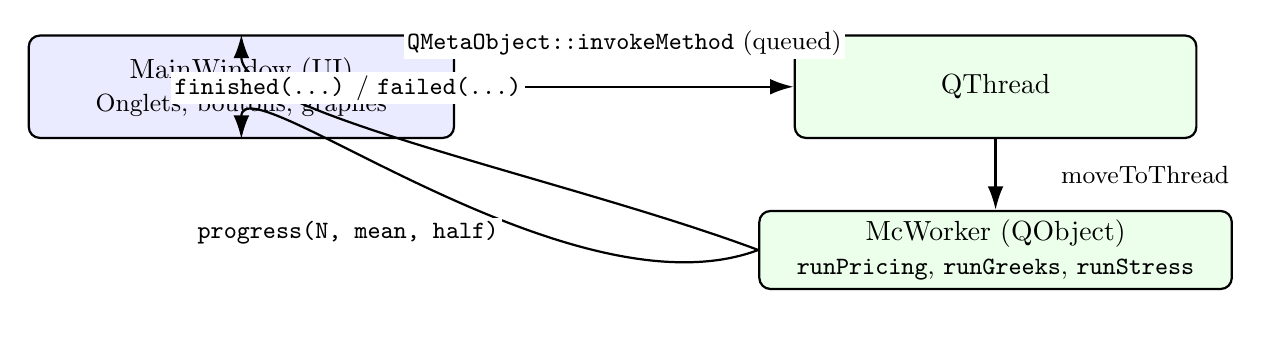
\begin{tikzpicture}[node distance=1.6cm]
\node[ui, minimum width=5.4cm, minimum height=1.3cm] (mw) {MainWindow (UI)\\\small Onglets, boutons, graphes};
\node[worker, right=4.3cm of mw, minimum width=5.1cm, minimum height=1.3cm] (thr) {QThread};
\node[worker, below=0.9cm of thr, minimum width=6.0cm] (wk) {McWorker (QObject)\\\small \code{runPricing}, \code{runGreeks}, \code{runStress}};

% appels
\draw[arrow] (mw.east) -- (thr.west);
\node[smalllab] at ($(mw.east)!0.5!(thr.west) + (0,0.55)$) {\code{QMetaObject::invokeMethod} (queued)};

\draw[arrow] (thr.south) -- (wk.north);
\node[smalllab] at ($(thr.south)!0.5!(wk.north) + (1.9,0)$) {moveToThread};

% retours (labels séparés et décalés)
\draw[arrow] (wk.west) .. controls +(-2.4,0.9) and +(0,-1.0) .. (mw.north);
\node[smalllab] at ($(wk.west)!0.55!(mw.north) + (-1.6,0.55)$) {\code{finished(...)} / \code{failed(...)}};

\draw[arrow] (wk.west) .. controls +(-2.4,-0.9) and +(0,1.0) .. (mw.south);
\node[smalllab] at ($(wk.west)!0.55!(mw.south) + (-1.6,-0.55)$) {\code{progress(N, mean, half)}};
\end{tikzpicture}
\caption{Threading : l’UI ne bloque jamais; le \emph{Worker} tourne dans un \code{QThread}, les retours se font par signaux.}
\end{figure}

\subsection{Chaîne Validation (tests enchaînés)}
\begin{figure}[H]\centering
\begin{tikzpicture}[node distance=0.8cm]
\node[calc] (t1) {Pricing vs \bs: \(\text{BS}\in\text{\ci}\)};
\node[calc, right=1.6cm of t1] (t2) {Convergence: pente \(\approx -1/2\)};
\node[calc, right=1.6cm of t2] (t3) {Greeks vs \bs: \(|z|_{\max}\le 2\)};
\node[calc, right=1.6cm of t3] (t4) {Stress (CRN): \(\mathrm{Var}(\mathrm{P\&L}) \ll \mathrm{Var}(P)\)};
\node[calc, right=1.6cm of t4] (t5) {Save/Load JSON: idempotence};
\draw[arrow] (t1) -- (t2);
\draw[arrow] (t2) -- (t3);
\draw[arrow] (t3) -- (t4);
\draw[arrow] (t4) -- (t5);
\end{tikzpicture}
\caption{Le bouton \emph{Run all tests} déclenche la séquence; chaque étape connecte/déconnecte proprement ses signaux.}
\end{figure}

\section{Blocs de la phase 3}

\subsection*{Bloc 1 — UI Qt, onglets}
\paragraph{But de la page} Offrir une navigation claire par \code{QTabWidget} :
\begin{enumerate}[leftmargin=*]
  \item \textbf{Market\_Instrument} : $S_0, r, q, \sigma$ et instrument $(K,T,$ call/put$)$.
  \item \textbf{Pricing} : bouton \emph{Run MC}, résultats (prix, SE, \ci, \(N_{\rm eff}\), temps), graphe de convergence.
  \item \textbf{Greeks} : méthode (BRV/PW/LRM), options CRN/antithétiques, bumps, bar chart.
  \item \textbf{Stress} : sliders chocs \(\Delta S\%\), \(\Delta\sigma\) (pts), \(\Delta r\) (bps), \(\Delta T\) (jours), P\&L \mc\ vs Taylor.
  \item \textbf{Validation} : tableau des tests, log détaillé.
\end{enumerate}

\subsection*{Bloc 2 — Lancer \mc\ sans bloquer l’UI}
\paragraph{But de la page} Déporter les calculs dans \code{McWorker} (dans un \code{QThread}). Publier \code{progress(N, mean, halfwidth95)} pour alimenter le graphe; conclure via \code{finished(price, se, ci\_low, ci\_high, N\_eff, elapsed\_ms)}.

\subsection*{Bloc 3 — Onglet Pricing}
\paragraph{But de la page} Calculer le prix \mc\ d’un vanille européen et visualiser la \textbf{convergence} vers la valeur \bs.

\paragraph{Éléments de la page}
\begin{itemize}[leftmargin=*]
  \item \textbf{Bouton \emph{Run MC}} : crée un \code{McConfig} (target, batch, tol, steps, seed), lance \code{runPricing}.
  \item \textbf{Panneau Résultats} : \emph{Price}, \emph{SE}, \emph{CI Low/High}, \emph{Number eff}, \emph{Elapsed}.
  \item \textbf{Graphe Convergence} : moyenne (orange), bande \ci\ (bleu), référence \bs\ (vert), dernier point (violet).
\end{itemize}

\paragraph{Théorie déclenchée}
Pour un call/put européen sous GBM :
\[
\hat{P}_N=\frac{1}{N}\sum_{i=1}^N e^{-rT}\Phi(S_T^{(i)}),\qquad
\mathrm{SE}=\frac{\hat{\sigma}}{\sqrt{N}},\qquad
\text{\ci}=[\hat{P}_N\pm 1.96\,\mathrm{SE}].
\]

\paragraph{Capture} \imgfull{pricing.png}

\subsection*{Bloc 4 — Onglet Greeks}
\paragraph{But de la page} Estimer \(\Delta,\) Vega, \(\Gamma,\rho,\Theta\) avec un bon compromis biais/variance.

\paragraph{Éléments de la page}
\begin{itemize}[leftmargin=*]
  \item \textbf{Méthode} : BRV (bump-and-revalue), PW (pathwise), LRM (likelihood ratio).
  \item \textbf{Options} : CRN, Antithetic variates; \emph{Bumps} \(\varepsilon\) pour \(S_0,\sigma,r,T\).
  \item \textbf{Output} : valeurs et bar chart.
\end{itemize}

\paragraph{Théorie déclenchée}
\begin{itemize}[leftmargin=*]
  \item \textbf{BRV} : différences centrées (CRN \(\Rightarrow\) variance réduite).
  \item \textbf{PW} : \(\Delta = \mathbb{E}[\partial \text{payoff}/\partial S_0]\) si la dérivée existe.
  \item \textbf{LRM} : dérivée de la densité (utile pour Vega sans bump).
\end{itemize}

\paragraph{Capture} \imgfull{greeks.png}

\subsection*{Bloc 5 — Onglet Stress Testing}
\paragraph{But de la page} Mesurer une \textbf{P\&L} sous chocs et la comparer à l’approximation \textbf{Taylor} d’ordre 2.

\paragraph{Éléments de la page}
\begin{itemize}[leftmargin=*]
  \item \textbf{Sliders} : \(\Delta S\) (\%), \(\Delta\sigma\) (pts), \(\Delta r\) (bps), \(\Delta T\) (jours).
  \item \textbf{AutoRun} : déclenche \code{runStress} avec \emph{debounce}.
  \item \textbf{Graphe} : pile Taylor (\(\Delta, \frac12\Gamma(\Delta S)^2, \text{Vega}\cdot \Delta\sigma, \rho\cdot\Delta r\)) et barre \mc.
\end{itemize}

\paragraph{Théorie déclenchée}
\[
\mathrm{P\&L} \approx \Delta\cdot \Delta S + \tfrac12 \Gamma (\Delta S)^2 + \text{Vega}\cdot \Delta\sigma + \rho \cdot \Delta r.
\]
Avec \textbf{CRN}, prix \textit{base} et \textit{stressé} partagent les mêmes tirages \(\{Z_k\}\) \(\Rightarrow\) variance de \(\mathrm{P\&L}\) fortement réduite.

\paragraph{Capture} \imgfull{stress.png}

\subsection*{Bloc 6 — Sauvegarde / Rechargement}\label{sec:bloc6}
\paragraph{But de la page} Rendre les scénarios \textbf{reproductibles} et partageables via un JSON lisible.

\paragraph{Fichier JSON}
\begin{lstlisting}[language=,basicstyle=\ttfamily\small]
{
  "market": {"S0":100,"r":0.02,"q":0.0,"sigma":0.2},
  "instrument": {"type":"call","K":100,"T":1.0},
  "mc": {"seed":42,"n_paths_target":400000,"batch_size":100000,
         "tolerance":-1,"n_steps":1,"use_antithetic":true,"use_crn":true},
  "ui": {"last_tab":"Pricing"}
}
\end{lstlisting}

\paragraph{Schéma}
\begin{figure}[H]\centering
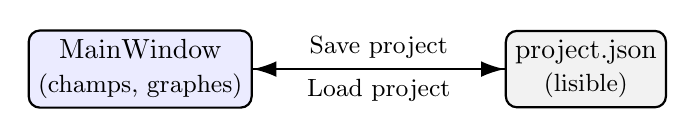
\begin{tikzpicture}[node distance=2cm]
\node[ui] (uiw) {MainWindow\\\small (champs, graphes)};
\node[file, right=3.2cm of uiw] (json) {project.json\\\small (lisible)};
\draw[arrow] (uiw) -- node[above,small]{Save project} (json);
\draw[arrow] (json) -- node[below,small]{Load project} (uiw);
\end{tikzpicture}
\caption{Sauvegarde/reload des paramètres et du dernier onglet visité.}
\end{figure}

\subsection*{Bloc 7 — Tests \& Validation}
\paragraph{But de la page} Proposer un bouton unique qui vérifie toute la chaîne (pricing, pente, greeks, CRN, save/load).

\paragraph{Règles d’acceptation}
\begin{enumerate}[leftmargin=*]
  \item \textbf{Pricing vs \bs} : le \bs\ est inclus dans l’intervalle \ci.
  \item \textbf{Greeks vs \bs} : \( \max |z|\le 2 \) (moyenne \mc\ vs \bs, SE par réplicas).
  \item \textbf{Stress (CRN)} : \(\mathrm{Var}(\mathrm{P\&L}) \ll \mathrm{Var}(P)\).
  \item \textbf{Convergence} : pente \(\log(\text{halfwidth})\) vs \(\log N\) proche de \(-\tfrac12\).
  \item \textbf{Save/Load} : re-pricing identique (\(|\Delta|\le 10^{-9}\)).
\end{enumerate}

\paragraph{Capture} \imgfull{validation.png}

\section{Processus détaillés (TikZ)}

\subsection{Pipeline Pricing \mc}
\begin{figure}[H]\centering
\resizebox{0.95\linewidth}{!}{%
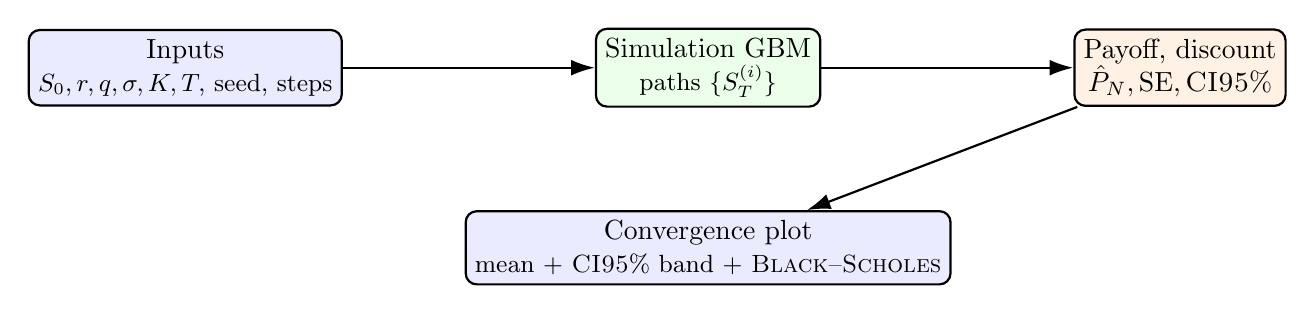
\begin{tikzpicture}[node distance=0.5cm]
\node[ui] (in) {Inputs\\\small \(S_0,r,q,\sigma,K,T,\) seed, steps};
\node[worker, right=3.2cm of in] (sim) {Simulation GBM\\\small paths \(\{S_T^{(i)}\}\)};
\node[calc, right=3.2cm of sim] (agg) {Payoff, discount\\ \(\hat P_N, \mathrm{SE}, \ci\)};
\node[ui, below=1.3cm of sim] (plot) {Convergence plot\\\small mean + \ci\ band + \bs};
\draw[arrow] (in) -- (sim);
\draw[arrow] (sim) -- (agg);
\draw[arrow] (agg) -- (plot);
\end{tikzpicture}%
}
\caption{Chaîne de pricing \mc.}
\end{figure}


\subsection{Greeks (BRV/PW/LRM)}
\begin{figure}[H]\centering
\resizebox{0.95\linewidth}{!}{%
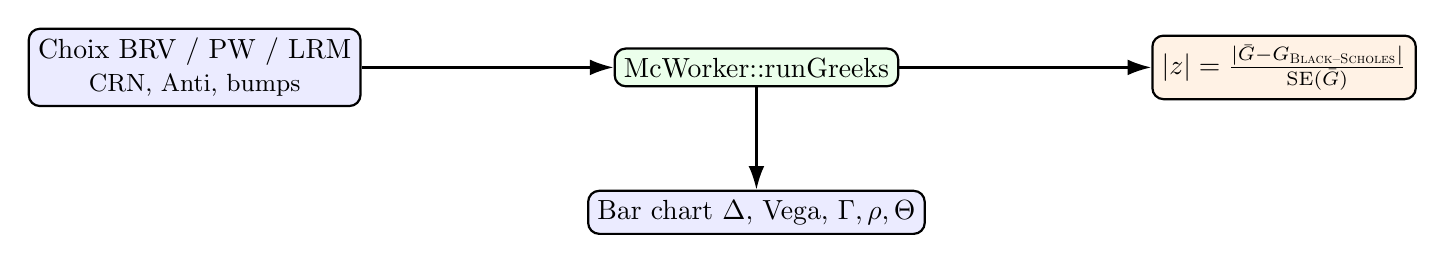
\begin{tikzpicture}[node distance=0.5cm]
\node[ui] (meth) {Choix BRV / PW / LRM\\\small CRN, Anti, bumps};
\node[worker, right=3.2cm of meth] (calcg) {McWorker::runGreeks};
\node[calc, right=3.2cm of calcg] (z) {\(|z|=\frac{|\bar{G}-G_{\bs}|}{\mathrm{SE}(\bar G)}\)};
\node[ui, below=1.3cm of calcg] (bar) {Bar chart \(\Delta,\) Vega, \(\Gamma,\rho,\Theta\)};
\draw[arrow] (meth) -- (calcg);
\draw[arrow] (calcg) -- (z);
\draw[arrow] (calcg) -- (bar);
\end{tikzpicture}%
}
\caption{Calcul des greeks et comparaison \bs.}
\end{figure}


\subsection{Stress avec CRN}
\begin{figure}[H]\centering
\resizebox{0.95\linewidth}{!}{%
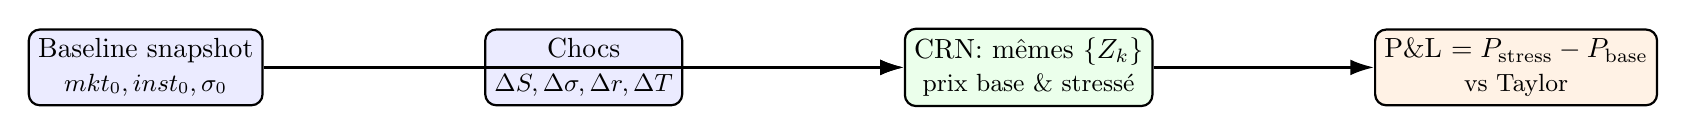
\begin{tikzpicture}[node distance=1.1cm]
\node[ui] (snap) {Baseline snapshot\\\small \(mkt_0, inst_0, \sigma_0\)};
\node[ui, right=2.8cm of snap] (shock) {Chocs\\\small \(\Delta S,\Delta\sigma,\Delta r,\Delta T\)};
\node[worker, right=2.8cm of shock] (crn) {CRN: mêmes \(\{Z_k\}\)\\\small prix base \& stressé};
\node[calc, right=2.8cm of crn] (pl) {P\&L \(=P_{\text{stress}}-P_{\text{base}}\)\\\small vs Taylor};
\draw[arrow] (snap) -- (crn);
\draw[arrow] (shock) -- (crn);
\draw[arrow] (crn) -- (pl);
\end{tikzpicture}%
}
\caption{Stress avec Common Random Numbers.}
\end{figure}


\section{Description détaillée des pages (+ théorie derrière les boutons)}

\subsection{Market\_Instrument}
\imgfull{market_instrument.png}
\paragraph{But de la page} Saisir les paramètres de marché et l’instrument de base.
\paragraph{Ce qu’on voit}
\begin{itemize}[leftmargin=*]
  \item Bloc \textbf{Market} : \(S_0\) (spot), \(r\) (taux), \(q\) (div), \(\sigma\) (vol).
  \item Bloc \textbf{Instrument} : \(K\) (strike), \(T\) (maturité, années), \textit{Type} (Call/Put).
  \item Boutons \textbf{Reset}, \textbf{Defaults}, \textbf{Save/Load project}.
\end{itemize}
\paragraph{Théorie/boutons}
\begin{itemize}[leftmargin=*]
  \item \textbf{Defaults} charge un set cohérent pour tester la chaîne complète.
  \item \textbf{Save/Load} sérialise la configuration (\S\ref{sec:bloc6}).
\end{itemize}

\subsection{Pricing}
\imgfull{pricing.png}
\paragraph{But de la page} Lancer un pricing \mc, suivre la convergence et comparer au prix \bs.
\paragraph{Boutons \& panneaux}
\begin{itemize}[leftmargin=*]
  \item \textbf{Run MC} lance \code{runPricing}. La moyenne par batch nourrit le graphe en direct (\code{progress}).
  \item \textbf{MC Config} : \emph{Target}, \emph{Batch}, \emph{Tol} (SE target si $>0$), \emph{Steps}, \emph{Seed}.
  \item \textbf{Legend} : code couleur \mc/\ci/\bs/dernier point.
\end{itemize}
\paragraph{Théorie}
Rappel \(\mathrm{SE}\propto 1/\sqrt{N}\). En Validation, la pente \(\approx-1/2\).

\subsection{Greeks}
\imgfull{greeks.png}
\paragraph{But de la page} Afficher les sensibilités principales avec la méthode choisie.
\paragraph{Boutons \& options}
\begin{itemize}[leftmargin=*]
  \item \textbf{Compute Greeks} : appelle \code{runGreeks}.
  \item \textbf{BRV}/\textbf{PW}/\textbf{LRM} : trois estimateurs complémentaires.
  \item \textbf{CRN}/\textbf{Anti} : réduction de variance.
\end{itemize}
\paragraph{Théorie}
Comparaison aux formules \bs; \(z\)-scores via réplicas indépendants.

\subsection{Stress}
\imgfull{stress.png}
\paragraph{But de la page} Visualiser P\&L \mc\ sous chocs et sa décomposition de Taylor.
\paragraph{Boutons \& graphe}
\begin{itemize}[leftmargin=*]
  \item \textbf{Sliders} pilotent les chocs; \textbf{AutoRun} applique un \emph{debounce} avant \code{runStress}.
  \item \textbf{Barres Taylor} : \(\Delta\cdot\Delta S\), \(\frac12\Gamma(\Delta S)^2\), \(\text{Vega}\cdot\Delta\sigma\), \(\rho\cdot\Delta r\).
  \item \textbf{Barre MC} : P\&L simulée avec CRN.
\end{itemize}
\paragraph{Théorie}
Le CRN fait chuter \(\mathrm{Var}(P_{\text{stress}}-P_{\text{base}})\) car la corrélation est proche de 1.

\subsection{Validation}
\imgfull{validation.png}
\paragraph{But de la page} Fournir un bouton unique \emph{Run all tests} pour valider la chaîne.
\paragraph{Boutons \& tableau}
\begin{itemize}[leftmargin=*]
  \item \textbf{Run all tests} enchaîne les 5 tests (prix, pente, greeks, CRN, save/load).
  \item \textbf{Table} : Test, métrique, valeur, seuil, verdict; \textbf{Log} détaille les nombres.
\end{itemize}

\section{Résultats (interprétation des figures)}
\subsection{Pricing — résultats}
\imgfull{pricing_res.png}
On observe un prix \mc\ \(\hat P\approx 2.149\) avec \(\mathrm{SE}\simeq 2.76\times10^{-3}\). Le prix \bs\ \(P_{\bs}\approx 2.1451\) est \emph{dans} l’intervalle \ci, ce qui valide le simulateur et le discount. La bande \ci\ se resserre comme \(1/\sqrt{N}\).

\subsection{Greeks — résultats}
\imgfull{greeks_res.png}
Pour la configuration donnée:
\[
(\Delta,\ \text{Vega},\ \Gamma,\ \rho,\ \Theta)\ \approx\ (0.844,\ 22.18,\ 0.1199,\ 82.29,\ -1.8866).
\]
Avec CRN et un bump \(\sigma\) \emph{clampé} (p.ex. \(10^{-3}\)), les \(z\)-scores restent modestes; \(\max|z|\ll 2\).

\subsection{Stress — résultats}
\imgfull{stress_res.png}
La barre \mc\ (grisée) est comparée à la pile Taylor (couleurs). Pour \(\Delta S>0\), la brique \(\Delta\cdot\Delta S\) domine; \(\Gamma\) devient visible pour grands \(|\Delta S|\). \(\text{Vega}\) et \(\rho\) répondent à \(\Delta\sigma\) et \(\Delta r\). CRN stabilise la P\&L.

\subsection{Validation — résultats}
\imgfull{validation_res.png}
\begin{itemize}[leftmargin=*]
  \item \textbf{Pricing vs \bs} : PASS (\bs\ dans \ci).
  \item \textbf{Convergence} : pente \(\approx -0.501 \in[-0.60,-0.40]\).
  \item \textbf{Greeks vs \bs} : \(\max|z|\approx 0.42 \le 2\).
  \item \textbf{Stress (CRN)} : \(\mathrm{Var(P\&L)}/\mathrm{Var}(P)\) très faible.
  \item \textbf{Save/Load} : \(|P_2-P_1|=0\) (à \(\le 10^{-9}\)).
\end{itemize}

\section{Problèmes rencontrés \& solutions}

\begin{enumerate}[leftmargin=*]
  \item \textbf{Segfault dans la variance} (lecture hors borne pour \(n<2\)). \fix{implémentation Welford, garde \(n<2\to 0\).}
  \item \textbf{Segfaults intermittents (AddressSanitizer)} dus à signaux encore émis après destruction / doubles connexions. \fix{cycle Worker strict (\code{start/stop}), \code{Qt::UniqueConnection}, \code{disconnect()} explicites, état dans \code{std::shared\_ptr}.}
  \item \textbf{Erreur de copie \code{McConfig}} (operator= supprimé via champs \code{const}). \fix{stocker uniquement les \emph{scalaires} et reconstruire \code{McConfig} à la volée.}
  \item \textbf{Stress (CRN) FAIL} selon chocs/seed/steps. \fix{\code{onSnapBaseline()}, mêmes RNG pour base/stress, même \#steps, cas \(T=0\) géré, chocs par défaut si sliders nuls.}
  \item \textbf{Greeks instables (Vega/Theta)} pour bump \(\sigma\) trop grand. \fix{clamp \(\varepsilon_\sigma \approx 10^{-3}\), CRN, réplicas indépendants.}
  \item \textbf{Fuites QtCharts} (objets sans parent). \fix{parents systématiques pour \code{QChart}, séries, axes, \code{QChartView}, ou insertion via layout parenté.}
  \item \textbf{Fuite \code{libdbus} \(\sim\)1KB} à l’arrêt (externe). \emph{Note} : inoffensif; possible suppression via LSAN.
  \item \textbf{Logs \code{QString::arg} mal formés}. \fix{\code{QString::asprintf} partout pour éviter les erreurs d’index.}
  \item \textbf{Réentrance Validation}. \fix{enchaînement strict (disconnect/stop avant test suivant).}
\end{enumerate}


\end{document}
